page2
Proposed Research Contribution




\markup{RI: I modified this based on PPT used on previous meeting}

\begin{figure}[h!]
	\centering
	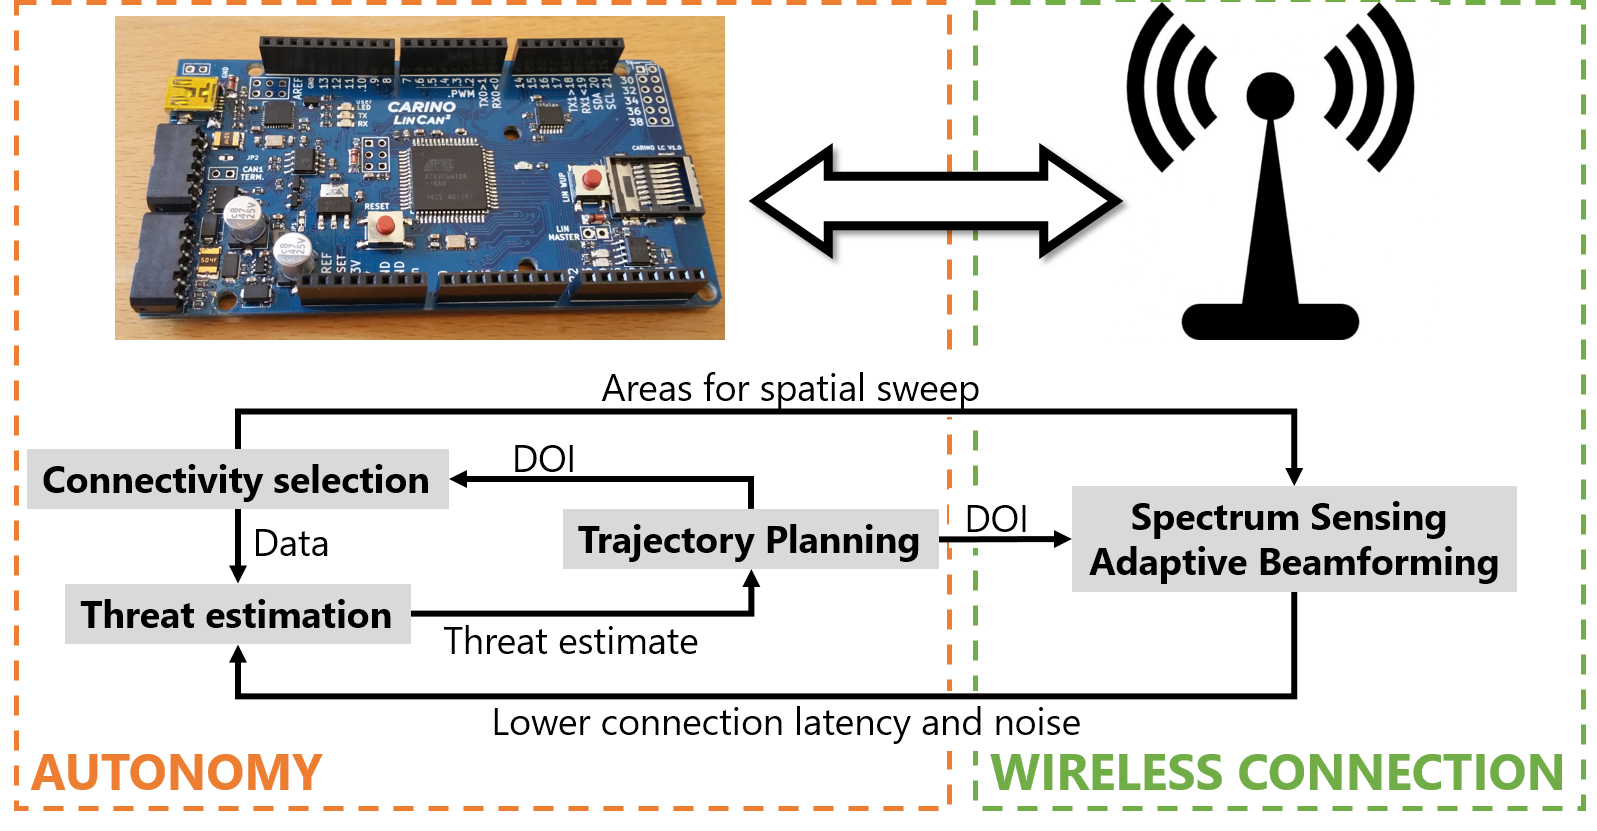
\includegraphics[width=0.7\columnwidth]{\figpath/project-block}
	\caption{A block diagrammatic illustration of the proposed technical approach.}
	\label{fig-project-block}
\end{figure}

\textbf{Scope of the project:} We focus on how the wireless imperfections affect the control algorithm of lane keeping using BSM
messages information from DSRC/WAVE standard in various scenarios. 
commands. 

\textbf{Terminology:} We refer to the vehicle implementing the proposed algorithms as the 
\mydef{own vehicle}; to other possible connections, including other vehicles, smart 
infrastructure, and personal gadgets as \mydef{data nodes} or \mydef{nodes}; and to
all collision threats, such as these nodes as well as static obstacles, as \mydef{other entities}.
%

The proposed technical approach consists of the following inter-related aspects 
(see \fig{fig-project-block}):
%
\begin{enumerate}[1.]
	\listformat
	\item \textbf{Transmission Imperfections}
	
	\item \textbf{Heartbeat message BSM }
	
	
	\item{\textbf{Feedback Channels}}
	\item \textbf{Power control on emergency channel in DSRC }
	
	The DSRC define  two emergency channel. The channel 172 is short range for accident avoidance and mitigation and channel 184 is long range and focus on road intersection collision mitigation. The proposal is to use two different power control strategy to maintain  range of each emergency channel on a useful range to avoid interference.  
	
	\item \textbf{Robustness of control laws to imperfect communications:} 
	All vehicles are represented by particle dynamical models.
	The control problem for the own vehicle is formulated as a problem of
	satisfying linear temporal logic (LTL) specifications under imperfect 
	information. These specifications will encode the primary requirement
	of collision avoidance, as well as compliance with additional traffic
	regulations (e.g. maximum speed). The control problem for the own vehicle 
	treats the data about positions and velocities of other vehicles as ``sensor 
	measurements.'' These data are inherently uncertain due to navigational 
	uncertainty of each vehicle. Furthermore, these data are transmitted over 
	imperfect communication channels that involve latency, dropped packets, and 
	re-transmissions. The proposed work will characterize the robustness of control 
	laws under such imperfect information, namely, the dependence of the 
	probability of failure to satisfy the given LTL specifications on the 
	nature of imperfections in data.
\end{enumerate}
